\chapter{Crypto.Types.Nonces}
This package provides a generic type \texttt{Nonce} with related
procedures and functions. "A nonce is a cryptographic input value
which must never repeat within a given context"
\cite{DBLP:conf/isw/Zenner09}. Nonces are important for the security
of many cryptographic building blocks, such as block ciphers, modes of
operations, as well as message authentication codes
\cite{DBLP:conf/isw/Zenner09}. For a message $M$ after encryption with
the same key but different nonce values $N_1\neq N_2$, we'll get with
great probability that $E_K(M,N_1)\neq E_K(M,N_2)$. The package is
specified in \texttt{Crypto.Types.Nonces}.


\section{Crypto.Types.Mutexes}
In order to avoid some confusions during the process of calculation by
different threads, a state value of type \texttt{Mutex\_Type}
(\texttt{Crypto.Types.Mutexes}) is used. We use this state value
combined with the data to indicate if the data is seized by some
thread. If yes, then the status is locked (owned is "true"), and the
other threads should wait until it's free. Mutex guarantees that only
one thread can process the resource at one time, and the other
threads, if more than one thread, should wait in a queue for the
resource. Another status is named released (owned is "false") if the
resource is hold by no thread (free state).

\begin{lstlisting}{}
  protected type Mutex_Type is
    entry Seize;
    procedure Release;
  private
    Owned : Boolean := False;
  end Mutex_Type;
\end{lstlisting}
This workflow is called rendezvous in Ada, in the above example they
interact indirectly through shared data. Rendezvous is similar to the
human situation when two people meet, they perform a transaction and
then go on independently \cite{Ada2005}.

%%%%%%%%%%%%%%%%%%%%%%%%%%%%%%%%%%%%%%%%%%%%%%%%%%%%%%%%%%%%%%%%%
%%%%%%%%%%%%%%%%%%%%%%%%%%%%%%%%%%%%%%%%%%%%%%%%%%%%%%%%%%%%%%%%%
\section{API}
\subsubsection*{Generic Part}
\begin{lstlisting}{}
  generic
    type Block is private;
\end{lstlisting}
\subsubsection*{Types}
\begin{lstlisting}{}
  type Nonce is abstract limited new
  					Fin.Limited_Controlled with private;
\end{lstlisting}
The term \texttt{Fin} represents \texttt{Ada.Finalization}.
\subsubsection*{Procedures}
\begin{lstlisting}{}
  overriding
  procedure Finalize(This : in out Nonce) is null;
  not overriding
  function Update(This: in out Nonce) return Block is abstract;
\end{lstlisting}
The \textbf{overriding} indicator confirms that we did indeed mean to
override the inherited procedure \texttt{Finalize()}, and the function
\texttt{Update()} is a new operation. Since the function is abstract,
it has no body and can not be called.\\

%%%%%%%%%%%%%%%%%%%%%%%%%%%%%%%%%%%%%%%%%%%%%%%%%%%%%%%%%%%%%%%%%
%%%%%%%%%%%%%%%%%%%%%%%%%%%%%%%%%%%%%%%%%%%%%%%%%%%%%%%%%%%%%%%%%

\section{Child Packages}
\subsection*{Nonces\_Ctr}
The most widespread deterministic generator is a simple counter. This
package is specified in \texttt{Crypto.Types.Nonces.Nonces\_Ctr}.

%%%%%%%%%%%%%%%%%%%%%%%%%%%%%%%%%%%%%%%%%%%%%%%%%%%%%%%%%%%%%%%%%

\subsubsection*{Generic Part}
\begin{lstlisting}{}
  generic
    with function Inc(B : in Crypto.Types.Nonces.Block)
   							return Crypto.Types.Nonces.Block;
\end{lstlisting}
The function \texttt{Inc()} is usually specified by users. It points
out how the counter value is updated, usually it is set to be
increased by one after each invocation.

%%%%%%%%%%%%%%%%%%%%%%%%%%%%%%%%%%%%%%%%%%%%%%%%%%%%%%%%%%%%%%%%%

\subsubsection*{Types}
\begin{lstlisting}{}
  type Nonce_Ctr is new N.Nonce with private;
\end{lstlisting}

%%%%%%%%%%%%%%%%%%%%%%%%%%%%%%%%%%%%%%%%%%%%%%%%%%%%%%%%%%%%%%%%%

\subsubsection*{Procedures}
\begin{lstlisting}{}
  procedure Initialize(This       : in out Nonce_Ctr;
                       File_Path  : in     String;
                       IV         : in     N.Block);
  procedure Initialize(This       : in out Nonce_Ctr;
  					   	  File_Path  : in     String);
\end{lstlisting}
The two procedures make both the initialization, the first one is used
usually at the first time to set a start value (IV), and specify a
file to store the nonces. The second procedure make the initialization
by recalling the nonce file.\\ 

\noindent\textbf{Exception:}\\  File  is  open  when  expected  to  be
closed:\quad  \texttt{Ada.IO\_Exceptions.Status\_Error}.\\ If  a wrong
file  name: \quad \texttt{Ada.IO\_Exceptions.Name\_Error}.

\hhline
\begin{lstlisting}{}
  overriding
  function Update(This : in out Nonce_Ctr) return N.Block;
\end{lstlisting}
It updates the nonce value by returning a new nonce value.

\hhline
\begin{lstlisting}{}
  overriding
  procedure Finalize(This : in out Nonce_Ctr);
\end{lstlisting}
It makes the finalization by checking whether the file is closed or
not. If the file is open, then close it.

\paragraph{Notice.}
As long as the number $\theta$ (the maximal number of nonces produced
by a generator) of nonces drawn is at most $2^\ell$ ($\ell$: the
length of nonce), the output of a counter-based generator is
guaranteed to be collision-free \cite{DBLP:conf/isw/Zenner09}.\\

%%%%%%%%%%%%%%%%%%%%%%%%%%%%%%%%%%%%%%%%%%%%%%%%%%%%%%%%%%%%%%%%%

\subsection*{Nonces\_Random}
The package is specified in
\texttt{Crypto.Types.Nonces.Nonces\_Random}. It returns randomly
generated value of specified length when a value of type
\texttt{Nonces\_Random} is requested. This random number generator
(RNG) does not maintain an inner state and therefore, does not need an
\texttt{Initialize()} function \cite{DBLP:conf/isw/Zenner09}. The RNG
is cryptographically secure.


\subsubsection*{Generic Part}
\begin{lstlisting}{}
  generic
    with function To_Block_Type(B: in Crypto.Types.Bytes)
    							return Crypto.Types.Nonces.Block;
\end{lstlisting}

%%%%%%%%%%%%%%%%%%%%%%%%%%%%%%%%%%%%%%%%%%%%%%%%%%%%%%%%%%%%%%%%%

\subsubsection*{Types}
\begin{lstlisting}{}
  type Nonce_Rand is new N.Nonce with private;
\end{lstlisting}

%%%%%%%%%%%%%%%%%%%%%%%%%%%%%%%%%%%%%%%%%%%%%%%%%%%%%%%%%%%%%%%%%

\subsubsection*{Procedures}
\begin{lstlisting}{}
  overriding
  function Update(This: in out Nonce_Rand) return N.Block;
\end{lstlisting}
This function updates the nonce value by returning a new random value.

%%%%%%%%%%%%%%%%%%%%%%%%%%%%%%%%%%%%%%%%%%%%%%%%%%%%%%%%%%%%%%%%%


\subsection*{Nonces\_Mixed\_1}
This is a mixed solution of the two approaches introduced above by
concatenating the random number and the counter, both of the length
$\ell_1$, into one output value of length $\ell$ with
$\ell=2\ell_1$. For every call to the function \texttt{Update()}, the
counter will be increased by one, and a new random number will be
generated. Obviously, this solution has a disadvantage of the
RNG-based solution, that when an RNG is required, there is a risk for
collisions. However, the collision probability and thus the nonce
length is reduced by the counter part
\cite{DBLP:conf/isw/Zenner09}. Figure 6.1 shows briefly how a nonce of
type \texttt{Nonces\_Mixed\_1} is processed.
\begin{figure}[h]
\centering
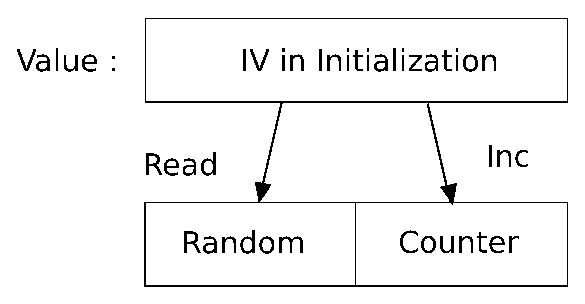
\includegraphics[scale=0.8]{./images/Nonce_Mixed_1}
\caption{The workflow of Nonce\_Mixed\_1.}
\end{figure}
\subsubsection*{Generic Part}
\begin{lstlisting}{}
generic
  Counter_Size: Positive := Block'Size / 16;
  with function To_Block_Type(Byte_Array:in Crypto.Types.Bytes)
   								return Crypto.Types.Nonces.Block;
  with function To_Bytes(Block: in Crypto.Types.Nonces.Block)
    								return Crypto.Types.Bytes;
\end{lstlisting}

%%%%%%%%%%%%%%%%%%%%%%%%%%%%%%%%%%%%%%%%%%%%%%%%%%%%%%%%%%%%%%%%%

\subsubsection*{Types}
\begin{lstlisting}{}
  type Nonce_Mixed_1 is new N.Nonce with private;
\end{lstlisting}

%%%%%%%%%%%%%%%%%%%%%%%%%%%%%%%%%%%%%%%%%%%%%%%%%%%%%%%%%%%%%%%%%

\subsubsection*{Procedures}
\begin{lstlisting}{}
  procedure Initialize(This : in out Nonce_Mixed_1; IV : in N.Block);
\end{lstlisting}
This procedure sets IV as the start value for the counter.

\hhline
\begin{lstlisting}{}
  overriding
  function Update(This : in out Nonce_Mixed_1) return N.Block;
\end{lstlisting}
This function increments the counter by one and stores the counter in
the second half of the nonce value. Then, it generates a new random
value and returns the concatenation: (half random and half counter)
random $\parallel$ counter.


%%%%%%%%%%%%%%%%%%%%%%%%%%%%%%%%%%%%%%%%%%%%%%%%%%%%%%%%%%%%%%%%%

\subsection*{Nonces\_Mixed\_2}
In this mixed solution, the initial vector IV will be stored to check
overflow. It separates the generation process into two steps. The
first step is the assignment of a random value to the first part of
the nonce. The second step is the update of the counter. At the end of
the update it checks the counter. If the counter overflows, then the
first step will be called once more. Figure \ref{Nonce2} shows how a
value of Nonces\_Mixed\_2 is generated.
\begin{figure}[h]
\centering
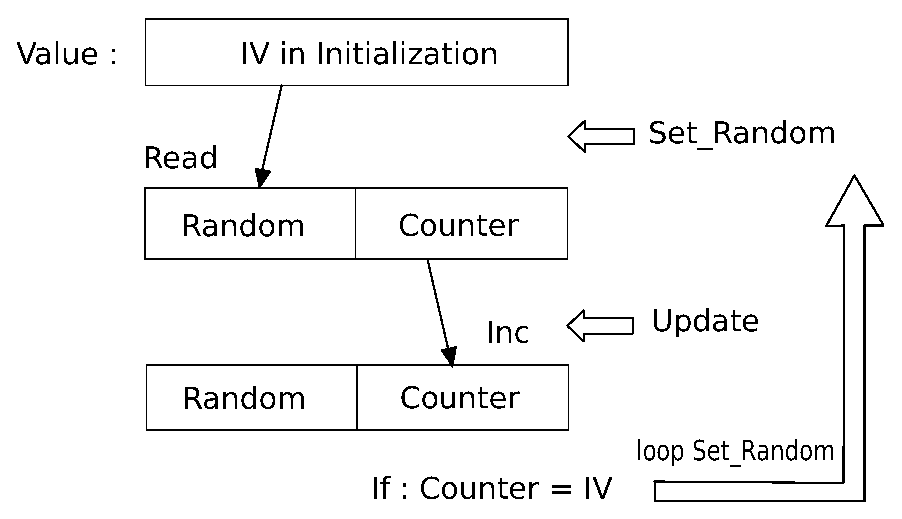
\includegraphics[scale=0.9]{./images/Nonce_Mixed_2}
\caption{The workflow of Nonces\_Mixed\_2.}\label{Nonce2}
\end{figure}

%%%%%%%%%%%%%%%%%%%%%%%%%%%%%%%%%%%%%%%%%%%%%%%%%%%%%%%%%%%%%%%%%

\subsubsection*{Generic Part}
\begin{lstlisting}{}
generic
  Counter_Size: Positive := Block'Size / 16;
  with function To_Block_Type(Byte_Array:in Crypto.Types.Bytes)
    								return Crypto.Types.Nonces.Block;
  with function To_Bytes(Block: in Crypto.Types.Nonces.Block)
    								return Crypto.Types.Bytes;
\end{lstlisting}

%%%%%%%%%%%%%%%%%%%%%%%%%%%%%%%%%%%%%%%%%%%%%%%%%%%%%%%%%%%%%%%%%

\subsubsection*{Types}
\begin{lstlisting}{}
  type Nonce_Mixed_2 is new N.Nonce with private;
\end{lstlisting}

%%%%%%%%%%%%%%%%%%%%%%%%%%%%%%%%%%%%%%%%%%%%%%%%%%%%%%%%%%%%%%%%%

\subsubsection*{Procedures}
\begin{lstlisting}{}
  procedure Initialize(This : in out Nonce_Mixed_2; IV : in N.Block);
\end{lstlisting}
It does the initialization and calls an internal procedure
\texttt{Set\_Random()} to generate a random value and store it in the
first half of the block. IV is assigned to the second half.

\hhline
\begin{lstlisting}{}
  overriding
  function Update(This : in out Nonce_Mixed_2) return N.Block;
\end{lstlisting}
The function \texttt{Update()} calls an internal function
\texttt{Inc()}, which increments the counter by one and stores the
counter in the second half of the block.

%%%%%%%%%%%%%%%%%%%%%%%%%%%%%%%%%%%%%%%%%%%%%%%%%%%%%%%%%%%%%%%%%%%
%%%%%%%%%%%%%%%%%%%%%%%%%%%%%%%%%%%%%%%%%%%%%%%%%%%%%%%%%%%%%%%%%%%
\newpage
\section{Example}
\subsubsection*{Nonce\_Ctr}
\begin{lstlisting}{}
  with Crypto.Types.Nonces;
  with Crypto.Types.Nonces.Nonces_Ctr;
  with Ada.Text_IO;
  with Ada.Directories;
  procedure Example_Nonces_Ctr is
    subtype Block is Natural range 0..255;
    function Inc(Item: Block) return Block is
         Result: Block := Item;
       begin
         Result := Result + 1;
         return Result;
    end Inc;
    package N is new Crypto.Types.Nonces(Block => Block);
    package Counter is new N.Nonces_Ctr(Inc => Inc);
    Nonce: Counter.Nonce_Ctr;
    B: Block := 0;
    Result : array(0..99) of Block;
    Distinct : Boolean := True;
  begin
    Counter.Initialize(This      => Nonce,
                       File_Path => "last_nonce.txt",
                       IV        => B);
    for i in Result'Range loop
        Result(i) := Counter.Update(Nonce);
    end loop;
    Counter.Finalize(Nonce);
    for i in Result'Range loop
        for j in (i+1)..Result'Last loop
            if Result(i) = Result(j) then
               Distinct := false;
            end if;
         end loop;
    end loop;
    Ada.Directories.Delete_File("last_nonce.txt");
    Ada.Text_IO.Put_Line(Distinct'Img);
  end Example_Nonces_Ctr;
\end{lstlisting}

%%%%%%%%%%%%%%%%%%%%%%%%%%%%%%%%%%%%%%%%%%%%%%%%%%%%%%%%%%%%%%%%%%%

\subsubsection*{Nonces\_Random}
\begin{lstlisting}{}
  with Crypto.Types.Nonces;
  with Crypto.Types.Nonces.Nonces_Random;
  with Crypto.Types; use Crypto.Types;
  with Ada.Text_IO;
  procedure Example_Nonces_Random is
     package N is new Crypto.Types.Nonces(Crypto.Types.B_Block128);
     package Rand is new N.Nonces_Random(Crypto.Types.To_B_Block128);
     Nonce: Rand.Nonce_Rand;
     Byte_Array: Crypto.Types.B_Block128 := (others => 0);
     Result : array(0..99) of Crypto.Types.B_Block128;
     Distinct : Boolean := True;
  begin
     for i in Result'Range loop
         Result(i) := Rand.Update(Nonce);
     end loop;
     for i in Result'Range loop
         for j in (i+1)..Result'Last loop
             if Result(i) = Result(j) then
                  Distinct := false;
             end if;
         end loop;
     end loop;
     Ada.Text_IO.Put_Line(Distinct'Img);
  end Example_Nonces_Random;
\end{lstlisting}
